\documentclass[a4paper,12pt]{article}

%%% Работа с русским языком
\usepackage{cmap}					          % поиск в PDF
\usepackage[T2A]{fontenc}			      % кодировка
\usepackage[utf8]{inputenc}               % кодировка исходного текста
\usepackage[english, russian]{babel}   % локализация и переносы

\usepackage{minted}

%%% Страница 
\usepackage{extsizes} % Возможность сделать 14-й шрифт
\usepackage{geometry}  
\geometry{left=20mm,right=20mm,top=25mm,bottom=30mm} % задание полей текста

\usepackage{titleps}      % колонтитулы
\newpagestyle{main}{
	\setheadrule{.4pt}                      
	\sethead{\CourseName}{}{\hyperlink{intro}{\;Назад к содержанию}}
	\setfootrule{.4pt}                       
	\setfoot{\CourseDate \; ФПМИ МФТИ}{}{\thepage} 
}      
\pagestyle{main}    % Устанавливает контитулы на странице


%%%  Текст
\setlength\parindent{0pt}         % Устанавливает длину красной строки 0pt
\sloppy                                        % строго соблюдать границы текста
\linespread{1.3}                           % коэффициент межстрочного интервала
\setlength{\parskip}{0.5em}                % вертик. интервал между абзацами
%\setcounter{secnumdepth}{0}                % отключение нумерации разделов
%\setcounter{section}{-1}         % Чтобы сделать нумерацию лекций с нуля
\usepackage{multicol}				          % Для текста в нескольких колонках
%\usepackage{soul}
\usepackage{soulutf8} % Модификаторы начертания


%%% Гиппер ссылки
\usepackage{hyperref}
\usepackage[usenames,dvipsnames,svgnames,table,rgb]{xcolor}
\hypersetup{				% Гиперссылки
	unicode=true,           % русские буквы в раздела PDF\\
	pdfstartview=FitH,
	pdftitle={Заголовок},   % Заголовок
	pdfauthor={Автор},      % Автор
	pdfsubject={Тема},      % Тема
	pdfcreator={Создатель}, % Создатель
	pdfproducer={Производитель}, % Производитель
	pdfkeywords={keyword1} {key2} {key3}, % Ключевые слова
	colorlinks=true,       	% false: ссылки в рамках; true: цветные ссылки
	linkcolor=blue,          % внутренние ссылки
	citecolor=green,        % на библиографию
	filecolor=magenta,      % на файлы
	urlcolor=NavyBlue,           % на URL
}

\usepackage{todonotes}


%%% Для формул
\usepackage{amsmath}          
\usepackage{amssymb}


%%%%%% theorems
\usepackage{amsthm}  % for theoremstyle

\theoremstyle{plain} % Это стиль по умолчанию, его можно не переопределять.
\newtheorem{theorem}{Теорема}[section]
\newtheorem{prop}[theorem]{Утверждение}
\newtheorem{lemma}{Лемма}[section]
\newtheorem{sug}{Предположение}[section]

\theoremstyle{definition} % "Определение"
\newtheorem{Def}{Определение}
\newtheorem{corollary}{Следствие}[theorem]
\newtheorem{problem}{Задача}[section]

\theoremstyle{remark} % "Примечание"
\newtheorem*{nonum}{Решение}
\newtheorem*{definition}{Def}
\newtheorem*{example}{Пример}
\newtheorem*{note}{Замечание}


%%% Работа с картинками
\usepackage{graphicx}                           % Для вставки рисунков
\graphicspath{{images/}{images2/}}        % папки с картинками
\setlength\fboxsep{3pt}                    % Отступ рамки \fbox{} от рисунка
\setlength\fboxrule{1pt}                    % Толщина линий рамки \fbox{}
\usepackage{wrapfig}                     % Обтекание рисунков текстом
\graphicspath{{images/}}                     % Путь к папке с картинками

\newcommand{\drawsome}[1]{            % Для быстрой вставки картинок
    \begin{figure}[h!]
            \centering
            \includegraphics[scale=0.7]{#1}
            \label{fig:first}
    \end{figure}
}
\newcommand{\drawsomemedium}[1]{
    \begin{figure}[h!]
            \centering
            \includegraphics[scale=0.45]{#1}
            \label{fig:first}
    \end{figure}
}
\newcommand{\drawsomesmall}[1]{
    \begin{figure}[h!]
            \centering
            \includegraphics[scale=0.3]{#1}
            \label{fig:first}
    \end{figure}
}


%%% облегчение математических обозначений
\newcommand{\R}{\mathbb{R}}
\newcommand{\N}{\mathbb{N}}
%\newcommand{\C}{\mathbb{C}}             % команда уже определена где-то)
\newcommand{\Z}{\mathbb{Z}}
\newcommand{\E}{\mathbb{E}}
\newcommand{\brackets}[1]{\left({#1}\right)}      % автоматический размер скобочек
% Здесь можно добавить ваши индивидуальные сокращения 

%%%%%%%%%%%%%%%%%%%%%%%%%%%

\usepackage[utf8]{inputenc} % Включаем поддержку UTF8
\usepackage[russian]{babel}  % Включаем пакет для поддержки русского языка
\usepackage{mathtools}
\usepackage{amssymb}
\usepackage{amsthm}
\usepackage{graphicx}
\usepackage{subcaption}\usepackage{caption}
\usepackage{svg}

\usepackage{listings}
\usepackage{xcolor}

\newcommand{\listingsttfamily}{\fontfamily{NotoSansMono-TLF}\big}
\newcommand*\lsin{\lstinline[columns=fixed, basicstyle=\fontsize{13}{13}\ttfamily]}

\lstset{
  language = [11]C++,
  backgroundcolor=\color{black!5}, % set backgroundcolor
  keywordstyle = \color{blue},
  columns = flexible
}

\usepackage{xpatch}
\xpatchcmd{\minted}{\VerbatimEnvironment}{\VerbatimEnvironment\let\itshape\relax}{}{}
\usepackage{tcolorbox}
\usepackage{etoolbox}
\BeforeBeginEnvironment{minted}{\begin{tcolorbox}[
                  leftrule=0.5pt,
                  rightrule=0.5pt,
                  toprule=0.5pt,
                  bottomrule=0.5pt,
                  boxsep=0pt,
                  left=0pt,
                  right=0pt,
                  top=-1.7pt,
                  bottom=-1.7pt
                  ]}%
\AfterEndEnvironment{minted}{\end{tcolorbox}}%

\definecolor{bg}{rgb}{0.95,0.95,0.95}

\newminted[cminted]{c}{
  numbersep=5pt,
  framesep=2mm,
  baselinestretch=1.2,
  bgcolor=bg,
  linenos}

% https://github.com/heia-fr/pygments-arm
\newminted[asmminted]{ARM}{ 
  numbersep=5pt,
  framesep=2mm,
  baselinestretch=1.2,
  bgcolor=bg,
  linenos}

\newmintinline[asmmint]{ARM}{}
\newmintinline[cppmint]{cpp}{}
\newmintinline[cmint]{c}{}
\newmintinline[bmint]{bash}{}
                  
\newcommand\round[1]{\left[#1\right]}

\tolerance=1
\emergencystretch=\maxdimen
\hyphenpenalty=10000
\hbadness=10000


%%% Всю шаблонную информацию можно менять тут
\newcommand{\FullCourseNameFirstPart}{\so{АРХИТЕКТУРА КОМПЬЮТЕРОВ И}}
\newcommand{\FullCourseNameSecondPart}{\so{ОПЕРАЦИОННЫЕ СИСТЕМЫ}}
\newcommand{\SchoolName}{ФПМИ}
\newcommand{\TrackName}{ПМИ}
\newcommand{\SemesterNumber}{III}
\newcommand{\LecturerInitials}{Андреев Александр Николаевич}
\newcommand{\AutherInitials}{Кирилл Афентьев}
\newcommand{\VKLink}{https://yandex.ru}
\newcommand{\GithubLink}{https://github.com/MIPT-Group/Lectures_Tex_Club}

\newcommand{\CourseName}{АКОС} %  Используется в преамбуле для создания названия предмета в верхнем контитуле   
\newcommand{\CourseDate}{Осень 2022}           %  Используется в преамбуле для создания даты в нижнем контитуле

\includeonly{lectures/lect06.tex}  % Чтобы скомпилировать только часть лекций

\begin{document}
    \begin{titlepage}
	\clearpage\thispagestyle{empty}
	\centering
	
	\textit{Федеральное государственное автономное учреждение \\
		высшего образования}
	\vspace{0.5ex}
	
	\textbf{Московский физико-технический институт
    \\
    (национальный исследовательский университет)}
	\vspace{20ex}
	
	\rule{\linewidth}{0.5mm}
	{\textbf{\FullCourseNameFirstPart}}
	\\
	{\textbf{\FullCourseNameSecondPart}}
	\rule{\linewidth}{0.5mm}
	
	\SemesterNumber\ СЕМЕСТР
	\\
	Физтех-школа: \textit{\SchoolName}
	\\
	Направление: \textit{\TrackName}
	\\
	Лектор: \textit{\LecturerInitials}
	\vspace{1ex}
	
	\begin{figure}[!ht]
		\centering
		
\includegraphics[width=0.5\textwidth]{mipt}
		\label{fig:mipt}
	\end{figure}
\begin{flushright}
	\noindent
	%\\
	%\href{\OverleafLink}{\textit{Проект на overleaf}}
	\\
\end{flushright}
	
	\vfill
	Долгопрудный, \CourseDate\ год.
	\pagebreak
	
\end{titlepage}
    \newpage
    \hypertarget{intro}{}
    \tableofcontents

    \section{Вводная лекция}
  \subsection{Операционная система}
  Операционная система -- абстракция, которая связывает различные компоненты компьютера и пользовательские программы.
  
  \subsection{Из каких компонент состоит компьютер?}
  \begin{itemize}
    \item Центральный процессор (CPU или ЦП)
    \item Чипсет и материнская плата
    \item Оперативная память (Random Access Memory = RAM)
    \item Накопители (HDD, SSD, NVMe)
    \item Аудиокарта
    \item Сетевая карта
    \item GPU
    \item Шина (PCI, I2C, ISA)
  \end{itemize}
  
  \subsubsection{Процессор}
  \begin{itemize}
    \item Исполняет команды или \textit{инструкции}
    \item Регистры -- самые быстрые доступные ячейки памяти
    \item Регистры определяют разрядность процессора
    \item Операндами могут быть либо константы, либо регистры, либо ссылки на память
  \end{itemize}
  
  \subsubsection{Оперативная память}
  \begin{itemize}
    \item Random Access Memory
    \item Адресное пространство -- непрерывный массив байт от $0$ до $2^N$, где $N$ -- разрядность процессора ($64$ бита)
    \item В реальности процессоры на текущий момент обычно адресуют не более $48$ бит ($256$ терабайт)
    \item Инструкции процессора расположены также в RAM -- архитектура Фон-Неймана
  \end{itemize}
  
  Сейчас оперативная память работает значительно медленнее процессора (доступ к RAM занимает несколько десятков инструкций процессора). Поэтому внутри процессора есть несколько уровней своей ``оперативной памяти'': L1, L2, L3. Они устроены немного иначе, чем оперативная память, и стоят очень дорого. Если запрашивается доступ к 1 байту, а затем к следующему байту, то второе считывание будет сделано не из оперативной памяти, а из кэша (L1/L2/L3, в зависимости от их наполнения). О том, почему есть несколько уровней кэша, будет рассказано в следующих лекциях.
  Из-за существования кэшей, нам выгодно, чтобы данные лежали ``рядом'' в памяти. Один из примеров: \href{https://levelup.gitconnected.com/c-programming-hacks-4-matrix-multiplication-are-we-doing-it-right-21a9f1cbf53}{ускорение умножения матриц}.
  
  \subsection{Немного ассемблера}
  Ассемблер -- это вид для человека, эти команды -- не процессорные инструкции. На современных процессорах Intel длина инструкции обычно занимает от 1 до 8 байт. В этом курсе будет рассмотрена только архитектура x86. В инструкцию зашивается вся нужная информация: используемые константы, используемые адреса памяти и т.д. Подробнее об этом будет рассказано позже.

\begin{asmminted}
mov rax, qword ptr [rax]
add rax, 2
mov rbx, 1
add rax, rbx
\end{asmminted}

\asmmint{rax}, \asmmint{rbx} -- это регистры процессора. Всего различных регистров общего назначения 16. \newline

Первая инструкция в этом коде берёт адрес регистра \asmmint{rax}, считывает его содержимое, и записывает в него же, в \asmmint{rax}. \newline
Вторая команда прибавляет к содержимому \asmmint{rax} $2$. \newline
Третья команда записывает в \asmmint{rbx} $1$. \newline
Четвертая команда прибавляет \asmmint{rbx} к \asmmint{rax}.
        
    \subsection{Мультизадачность}
    \begin{itemize}
      \item Мультизадачность -- способность системы исполнять несколько задач (процессов) одновременно
      \item Cooperative multitaksing -- процессы добровольно передают управление друг другу
      \item Preemptive multitasking -- процессы вытесянются ОС каждые несколько миллисекунд
    \end{itemize}
    
    Минус cooperative multitasking: если процесс завис, то он не передаст управление дальше, остается только reset.\newline
    Первая Windows, в которой появился multitasking, это Windows 95, до этого был singleprocess MS-DOS.
    
    \subsubsection{Суперскалярность}
    \begin{itemize}
      \item Параллелизм уровня инструкций
      \item Если две инструкции независимы друг от друга, их можно выполнить параллельно
      \item Каждая инструкция состоит из нескольких этапов: fetch, decode, execute, memory access, register write back
      \item CPU pipeline
    \end{itemize}
    Пример процессора без суперскалярности: российский Эльбрус, в котором одна инструкция процессора содержит несколько операций, которые выполняются параллельно. Такой принцип называется VLIW -- Very Long Instruction Word.
    
    \subsubsection{CPU pipeline}
    \begin{figure}[H]
    \centering
  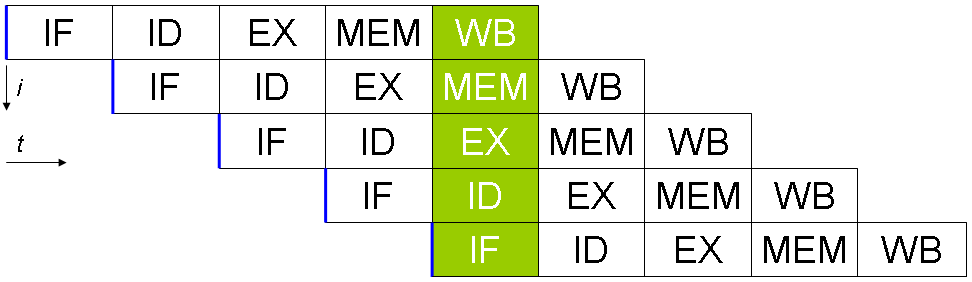
\includegraphics[width=\linewidth]{/Users/user/Downloads/cpu_pipeline.png}
  \caption{CPU pipeline}
  \label{fig:pipeline}
\end{figure}
    
    \subsubsection{Мультипроцессорность}
    \begin{itemize}
      \item Тактовая частота процессоров не растет примерно с 2005 года
      \item Поэтому современные процессоры обычно имеют несколько ядер
      \item \textit{Планировщик (scheduler)} ОС для каждого ядра процессора в каждый момент времени решает какой процесс будет запущен
      \item Возникают проблемы синхронизации
    \end{itemize}
    
    \subsection{Системные вызовы}
    \begin{itemize}
      \item Системные вызовы -- это интерфейс операционной системы для процессов
      \item ABI = application binary interface
      \item SystemV ABI
    \end{itemize}
    Системный вызов -- это очень дорогая операция. У каждой операционной системы свой ABI.
    
    \subsection{POSIX}
    \begin{itemize}
      \item Portable Operating System Interface
      \item Стандарт, описывающий интерфейс операционных систем
      \item Системные вызовы -- часть POSIX, но не все
      \item Например, POSIX описывает как должна быть устроена файловая система
    \end{itemize}
    Иными словами, POSIX -- это стандарт написания операционных систем. Windows -- не POSIX-совместимая система.
    
    \subsection{libc}
    \begin{itemize}
      \item Стандартная библиотека C
      \item Реализует системные вызовы в виде функций C
      \item Ещё куча всяких полезных функций :)
      \item Много реализаций, glibc одна из самых больших
    \end{itemize}
    POSIX определяет, как устроены системные вызовы в виде функций языка C.
    
    \subsubsection{Пример}
\begin{cminted}
int res = read(0, &buf, 1024);
if (res < 0) {
  char* err = strerror(errno);
  // ...
}
\end{cminted}
Функция \cmint{read} возвращает $-1$, если считать не получилось, в противном случае -- количество записанных байт. \newline
\cmint{errno} -- это глобальная переменная (внутри одного потока), в которой хранится последняя ошибка.\newline
Вернуть массив из функции сложно (о причинах будет рассказано в следующих лекциях), поэтому обычно мы просим не вернуть результат, а записать его по некоторому адресу в памяти.

    \subsection{Файловые дескрипторы}
    \begin{itemize}
      \item ``Everything is a file!''
      \item Каждый файл имеет своё имя (или \textit{путь})
      \item Преобразовывать имя файла на каждый сисколл дорого
      \item Сначала нужно получить файловый дескриптор (например, через сисколл \cmint{open})
      \item Все остальные операции без использования пути
    \end{itemize}
    Файловый дескриптор -- это число. Например, $0$ -- это \cmint{stdin}, $1$ -- это \cmint{stdout}, $2$ -- \cmint{stderr}.

    \section{Представление данных в компьютере}
  \subsection{Беззнаковые типы}
  \begin{itemize}
    \item Представляют из себя $N$-битные положительные числа на отрезке $[0, 2^N - 1]$
    \item Переполнение точно определено стандартом C (как сложение в $\mathbb{Z}_{2^N}$
    \item $1111+0001=10000=0$
  \end{itemize}
    
  \subsubsection{Endianess}
    \begin{itemize}
      \item Если $N = 64$, то $64 / 8 = 8$ байт нужно, чтобы представить число в памяти
      \item Если $N = 32$, то $32 / 8 = 4$ байта
      \item В какой последовательности хранить биты?
    \end{itemize}
    
    Есть 2 типа endianess:
    \begin{itemize}
      \item Little-endian: первые байты хранят младшие биты числа
      \item Big-endian: первые байты хранят старшие биты
    \end{itemize}
    Сейчас более распространен Little-endian.\\    Традиционно Big-endian используется в передаче данных по сети. Также первые процессоры использовали big-endian. PowerPC тоже использует big-endian.\\
    На некоторых arm-процессорах есть инструкция, позволяющая менять endian "на лету". 
    
\begin{figure}[h!]
  
\includegraphics[width=\linewidth]{/Users/user/Documents/endianess.png}
  \caption{Endianess}
  \label{fig:endianess}
\end{figure}

    
  \subsection{Выравнивание}
    \begin{itemize}
      \item Числа быстрее считываются процессором, если они лежат по адресам, кратным их размерам
      \item Например: \lsin{sizeof(int)} = 4 $\Rightarrow$ выравнивание по границе 4 байт
      \item \lsin{char} -- 1 байт
      \item \lsin{short} -- 2 байта
      \item \lsin{int} -- 4 байта
      \item \lsin{long long} -- 4 байта
    \end{itemize}
    
    Работа с выровненными данными происходит быстрее.\\
    Есть архитектуры, которые в принципе не позволяют читать по невыровненным адресам, например, arm. В процессорах Intel можно сделать так же.
    
  \subsubsection{Выравнивание структур}
    \begin{itemize}
      \item Члены структур располагаются рядом
      \item Но если им не хватает выравнивания, компилятор "добивает" структуру pad'ами
      \item Выравнивание структуры -- максимальное выравнивание среди всех выравниваний её членов
    \end{itemize}
    
  \subsection{Знаковые числа}
  \subsubsection{One's complemnt}
    \begin{itemize}
      \item $-A = BitwiseNot(A)$
      \item Диапазон: $[-2^{N - 1} + 1, 2^N - 1]$
    \end{itemize}
    Преимущество такого представления: естественным образом реализуется сложение чисел. Однако есть проблема.
    \begin{itemize}
      \item $-1 = 1110$
      \item $+1 = 0001$
      \item $1110 + 0001 = 1111 = -0$
    \end{itemize}
    Получается 2 представления нуля. Это порождает еще проблемы:
    \begin{itemize}
      \item $-1 = 1110$
      \item $+2 = 0010$
      \item $1110 + 0010 = \textcolor{red}{1}0000 = 0$
      \item Упс...
    \end{itemize}
  
  \subsubsection*{One's complement: end-around-carry}
    \begin{itemize}
      \item Бит переноса отправляется назад, чтобы всё исправить
      \item $1110 + 0010 = \textcolor{red}{1}0000 = 0 + \textcolor{red}{1} = 1$
    \end{itemize}
  
  \subsubsection*{One's complement: недостатки}
    \begin{itemize}
      \item Два представления для $0$: $0000 = +0$ и $1111 = -0$
      \item End-around-carry
      \item Зато сложение и вычитания одинаковое для знаковых и беззнаковых чисел (почти)!
    \end{itemize}
  
  \subsubsection{Two's complement}
    \begin{itemize}
      \item Определение отрицательных чисел: $A + (-A) = 0$
      \item Давайте каждому положительному число сопоставим отрицательное
      \item $-A = BitwiseNot(A) + 1$
      \item Одно представление нуля: $-0 = BitwiseNot(A) + 1 = 1111 + 1 = 0000 = +0$
      \item Диапазон чуть больше, чем у one's complement: $[-2^N, 2^N - 1]$
      \item Используется в современных процессорах
    \end{itemize}
    
    Теперь мы можем складывать знаковые и беззнаковые числа абсолютно одинаково.
  
  \subsubsection*{Two's complement: недостатки}
    \begin{itemize}
      \item Операции сравнения теперь сложные
      \item Умножение требует sign extension: $0010 = 00000010, 1000 = 11111000$
      \item ``Перекос'' диапазона представимых чисел
      \item \lsin{abs(INT_MIN)} = ???
    \end{itemize}
  
  \subsection{Действительные числа}
  \subsubsection{Числа с фиксированной точкой}
    \begin{itemize}
      \item $N$ бит на целую часть, $M$ бит на дробную
      \item Всегда одинаковая точность
      \item Операции легко реализуются
    \end{itemize}
  
  \subsubsection{Числа с плавающей точкой}
  Раньше процессоры имели отдельную плату для операций с числами с плавающей точкой.
    \begin{itemize}
      \item IEEE 754
      \item Стандарт 1985 года
    \end{itemize}
  
    Числа с плавающей точкой представлены 3 частями:
    \begin{itemize}
      \item Представление: $(-1)^S \times M \times 2^E$
      \item $S$ -- бит знака, $M$ -- мантисса, $E$ - экспонента
      \item \lsin{float} (single): $|S| = 1$, $|M| = 23$, $|E| = 8$
      \item \lsin{double}: $|S| = 1$, $|M| = 52$, $|E| = 11$
    \end{itemize}
  
  \subsubsection*{Нормализованные значения}
    \begin{itemize}
      \item $|E| \neq 0$ и $E \neq 2^{|E|} - 1$
      \item Экспонента хранится со смещением: $E_{real} = E - 2^{|E| - 1}$
      \item Мантисса имеет ``виртуальную 1'': $M_{real} = 1.mmmmmmm$
    \end{itemize}
    
  \subsubsection*{Денормализованные значения}
    \begin{itemize}
      \item $E = 0$
      \item $E_{real} = 1 - 2^{|E|} = 1$
      \item Это самые близкие к нулю числа и сам ноль ($0.0$ и $+0.0$)
    \end{itemize}
  
  \subsubsection*{Специальные значения}
    \begin{itemize}
      \item $E = 2^{|E| - 1}$
      \item Если $M = 0$, то число представляет собой бесконечное значение
      \item Если $M \neq 0$, то число -- NaN
      \begin{itemize}
        \item[$\circ$] Используются при операциях с неопределенным значением: например, $sqrt(X)$, $\log(X)$, $X < 0$
      \end{itemize}
    \end{itemize}
    
  \subsubsection*{Проблемы IEEE 754}
    \begin{itemize}
      \item При вычислениях накапливается ошибка
      \item Сложение и умножение неассоциативно
      \item Умножение недистрибутивно
      \item NaN $\neq$ NaN (???)
      \item $0.0$ и $+0.0$
    \end{itemize}
  
  Более подробно о числах с плавающей точкой можно прочитать \href{http://steve.hollasch.net/cgindex/coding/ieeefloat.html}{здесь}.
  
  \subsubsection{Decimals}
    \begin{itemize}
      \item Представляются в виде двух чисел: $N$ -- знаменатель, $M$ -- числитель
      \item Все операции реализуются через приведение к общему знаменателю
      \item $N$ и $M$ обычно используют длинную арифметику, поэтому в теории точность ограничена только оперативной памятью
      \item Используются в финансах
    \end{itemize}
  
  \subsection{Кодировки}
    \begin{itemize}
      \item Умеем оперировать числами, но как перевести числа в текст?
      \item Кодировки -- ``карты'', сопоставляющие наборы байт каким-то образом в символы
    \end{itemize}
  
  \subsubsection{Немного терминологии}
    \begin{itemize}
      \item Character -- что-то, что мы хотим представить
      \item Character set -- какое-то множество символов
      \item Coded character set (CCS) -- отображение символов в уникальные номера
      \item Code point -- уникальный номер какого-то символа
    \end{itemize}
    
  \subsubsection{ASCII}
    \begin{itemize}
      \item American Standard Code for Information Interchange, 1963 год
      \item 7-ми битная кодировка, то есть кодирует 128 различных символов
      \item Control characters: с $0$ по $31$ включительно, непечатные символы, мета-информация для терминалов
    \end{itemize}
  
  \subsubsection{Unicode}
    \begin{itemize}
      \item Codespace: $0$ до 0x10FFFF ($\sim$1.1 млн. code points)
      \item Code point'ы обозначаются как U+<число>
      \item $\aleph$ = U+2135
      \item $r$ = U+0072
      \item Unicode -- не кодировка: он не определяет как набор байт трактовать как characters
    \end{itemize}
  
  \subsubsection{UTF-32}
    \begin{itemize}
      \item Использует всегда 32 бита (4 байта) для кодировки
      \item Используется во внутреннем представлении строк в некоторых языках программирования (например, Python)
      \item Позволяет обращаться к произвольному code point'у строки за $\mathcal{O}(1)$
      \item BOM определяет little vs big-endian
    \end{itemize}
    Проблема: используется много места. Например, если мы пишем текст на английском, то под каждый символ будет выделено 4 байта, а можно было бы обойтись 1 (ASCII).
  
  \subsubsection{UTF-8}
    \begin{itemize}
      \item Unicode Transformation Format
      \item Определяет способ как будут преобразовываться code point'ы
      \item Переменная длина: от 1 байта (ASCII) до 4 байт
    \end{itemize}
    
    \begin{figure}[h!]
  \includegraphics[width=\linewidth]{/Users/user/Documents/utf8.png}
  \caption{UTF-8}
  \label{fig:utf8}
\end{figure}
  
  \subsubsection*{UTF-8 overlong encoding}
    \begin{itemize}
      \item $00100000$ = U+0020
      \item $11000000 \space 10100000$ = U+0020!
      \item overlong form или overlong encoding
      \item С точки зрения стандарта является некорректным представлением
    \end{itemize}
    \section{Файлы}
  \subsection{Файлы и директории}
    Файл -- это сущность, которая содержит данные и имеет имя.\\
    В Unix: Everything is a file!
  
  \subsubsection{Имя файла}
    \begin{itemize}
      \item Не более PATH\_MAX символов: 4 Кб на современных ОС, 256 байт для portability
      \item PATH\_MAX включает \textbackslash 0 в конце
      \item Разделитель пути -- /
      \item Части пути не более 255 символов каждая
    \end{itemize}
    
  \subsubsection{Имя директории}
    \begin{itemize}
      \item Абсолютный путь: начинается с корня (например, /Users/carzil/mipt)
      \item Относительный путь: вычисляется от текущей директории (например, carzil/mipt)
      \item . -- текущая директория (./carzil/mipt = carzil/mipt и ./carzil/./././mipt = ./carzil/mipt)
      \item .. -- директорий выше (/Users/carzil/mipt/.. = /Users/carzil)
    \end{itemize}
    
  \subsection{Файловые системы}
      \begin{itemize}
        \item Структура данных для организации хранения информации
        \item Метаданные -- информация о файле: дата последнего изменения, права доступа, создатель и так далее
        \item Работают поверх хранилища (HDD, SSD, NVMe)
        \item Хранилище традиционно разбивается на \textit{блоки}
        \item Размер блоков обычно 512 байт или 4Кб
      \end{itemize}
  
  \subsubsection{ext2}
    \begin{itemize}
      \item Linux, 1993 год
      \item inode -- физическое представление файла на диске: заголовок с метаинформацией + информация где он хранится
      \item Директории тоже хранятся в inode, так как директория -- файл!
    \end{itemize}

\begin{figure}[h!]
  \includegraphics[width=\linewidth]{/Users/user/Downloads/ext2_inode.png}
  \caption{inode}
  \label{fig:inode}
\end{figure}  
  
  \subsubsection{ext4}
    \begin{itemize}
      \item 2006 год
      \item Де-факто стандартная файловая система для Linux
      \item Журналируемая
      \item Для больших директорий используется HTree
    \end{itemize}
  
    Во времена ext2 была проблема: считалось, что жесткие диски живут долго и работают безотказно, однако на самом деле это было не так. При записи файла, например, могла произойти ошибка на жестком диске, и из-за этого ext2 ломалась. По этой причине в ext3 сделали журнал. Журнал -- это область на диске, в которую записываются логи всех операций, которые выполняются с данными. В ext3 в журнал записываются блоки, которые мы меняем на диске. Если в процессе изменения структуры данных файловой системы случился сбой диска, то в логи не будет записан маркер конца транзакции изменения файловой системы. И когда мы будем восстанавливать файловую систему по журналу, мы просто применим все записанные транзакции и получим какое-то её стабильное состояние. Также у нас есть возможность обратить изменения на диске. Это нам гарантирует, что если посреди операции возникла ошибка, мы не сломаем все данные, и сможем всё восстановить. Журналируемость можно отключить, благодаря этому файловая система будет работать быстрее. \\
    Еще одно отличие ext2 и ext3: есть директории, в которых находятся очень много файлов. Из-за этого поиск в таких директориях работает долго: нужно пробежаться по всем записям в inode и сравнить названия файлов с тем, что мы ищем. Поэтому в ext3 (и в ext4 соответственно) была создана структура данных HTree, которая хранит кэши файловых имен. Благодаря этому можно за амортизированное $\mathcal{O}(1)$ искать файлы в директориях. Использование HTree тоже можно отключить.
    
  \subsubsection{Другие файловые системы}
    \begin{itemize}
      \item FAT32
      \item NTFS (проприетарная, используется в Windows)
      \item ReiserFS (оптимизирует работу с большим количеством маленьких файлов)
      \item ZPS (может работать с несколькими устройствами)
    \end{itemize}
  
  \subsubsection{sysfs и procfs}
    \begin{itemize}
      \item ``Метафайловые системы''
      \item Не имеют никаких данных на диске, возвращают информацию напрямую из ядра Linux
      \item Часто используются, чтобы не добавлять новые сисколлы
    \end{itemize}

  \subsubsection{FUSE}
    \begin{itemize}
      \item Код файловой системы обычно расположен в ядре -- это неудобно
      \item FUSE = file system in userspace
    \end{itemize}
    Когда мы хотим поменять файл, мы сообщаем об этом операционной системе, а та, видя, что мы обращаемся к FUSE-файловой системе, передаст этот запрос процессу файловой системы.\\
    Пример использования: можно работать с файлами на удаленной машине, как будто они находятся локально на нашем компьютере.  В таком случае все изменения файловой системы будут пересылаться по сети. Это можно сделать при помощи SSHFS.
  
  \subsection{Файловые дескрипторы}
    \begin{itemize}
      \item Преобразование имени файла в inode -- очень дорогая операция, которая может требовать много обращений к диску
      \item Этот процесс ``кэшируют'' с помощью файловых дескрипторов
      \item Файловый дескриптор -- число больше 0
      \item Новый файловый дескриптор будет минимальным доступным числом
    \end{itemize}
  Благодаря файловым дескрипторам можно только один раз делать преобразование имени файла в inode (делая сисколл open). При этом привязка произойдет именно к inode, а не к имени файла.
    \begin{itemize}
      \item За каждым файловым дескриптором скрывается \href{https://elixir.bootlin.com/linux/v5.19.12/source/include/linux/fs.h#L925}{специальная структура} в ядре
      \item Указатель на inode, позиция в файле, флаги (чтения/запись/блокирование), различные локи и так далее
    \end{itemize}
  
    \subsubsection{Работа с данными файла}
\begin{lstlisting}[style=cpp]
#include <unistd.h>

int open(const char *pathname, int flags, mode_t mode);
ssize_t read(int fd, void *buf, size_t count);
ssize_t write(int fd, const void *buf, size_t count);
int close(int fd);
\end{lstlisting}
    
    \subsubsection{Работа с метаданными файла}
\begin{lstlisting}[style=cpp]
#include <sys/stat.h>

int stat(const char* path, struct stat* buf);
int fstat(int fd, struct stat *statbuf);
int lstat(const char* pathname, struct stat* statbuf);

struct stat {
  dev_t     st_dev;
  ino_t     st_ino;
  mode_t    st_mode;
  nlink_t   st_nlink;
  uid_t     st_uid;
  gid_t     st_gid;
  dev_t     st_rdev;
  off_t     st_size;
  blksize_t st_blksize;
  blkcnt_t  st_blocks;
  struct timespec st_atime/st_mtime/st_ctime;
};
\end{lstlisting}
    
    \subsubsection{Права доступа}
      \begin{itemize}
        \item rwx = \textbf{R}ead/\textbf{W}rite/e\textbf{X}ecute
        \item 9 бит, 3 группы; права владельца, права группы и права для остальных
        \item Часто записываются как числа в восьмиричной системе счисления
        \item $777_8 = 111111111_2$ = \lsin{rwxrwxrwx}
        \item $664_8 = 110100100_2$ = \lsin{rw-r--r--}
      \end{itemize}
    
    \subsubsection{Права доступа для директорий}
      \begin{itemize}
        \item r -- листинг директории
        \item w -- создание файлов внутри директории
        \item x -- возможность перейти в директорию (cd),  а также доступ к файлам
      \end{itemize}
    
    \subsubsection{Регулярные файлы}
      \begin{itemize}
        \item \lsin{S_ISREG(stat.st_mode)}
        \item Обычные файлы с данными
      \end{itemize}
    
    \subsubsection{Директории}
      \begin{itemize}
        \item \lsin{S_ISDIR(stat.st_mode)}
        \item Специальный API для чтения, обычные read/write не работают
        \item Создание и удаление: mkdir/rmdir
      \end{itemize}
    
\begin{lstlisting}[style=cpp]
#include <dirent.h>

struct dirent *readdir(DIR *dirp);

struct dirent {
  ino_t          d_ino;
  off_t          d_off;
  unsigned short d_reclen;
  unsigned char  d_type;
  char           d_name[256];
};

int closedir(DIR *dirp);
\end{lstlisting}
    
    \subsubsection{Символические ссылки}
      \begin{itemize}
        \item \lsin{S_ISLINK(stat.st_mode)}
        \item Аналог \lsin{std::weak_ptr} для inode
        \item Могут быть dangling: то есть ссылаться на файл, которого нет
        \item Отдельный тип файла
        \item Путь, на который она ссылается, записан в блоках
      \end{itemize}
    
    \subsubsection{Жесткие ссылки}
      \begin{itemize}
        \item Аналог \lsin{std::shared_ptr} для inode
        \item Только внутри одной файловой системы
        \item Если количество жестких ссылок стало равно 0, то inode становится свободной
        \item Не файл, а сущность файловой системы
      \end{itemize}
    
    \subsubsection{Символьные устройства (character device)}
      \begin{itemize}
        \item \lsin{S_ISCHR(stat.st_mode)}
        \item Устройства, из которых можно последовательно читать
        \item Клавиатура, звуковая карта, сетевая карта
        \item Такие файлы создаются драйверами ядра
      \end{itemize}
    
    \subsubsection{Блочные устройства (block device)}
      \begin{itemize}
        \item \lsin{S_ISBLC(stat.st_mode)}
        \item Разбиты на блоки одинакового размера
        \item Можно прочитать любой блок
        \item HDD, SSD, NAS
      \end{itemize}
    \section{Память}
  \subsection{Виртуальная память}
    Есть 2 проблемы: нужно выделить каждому процессу память, при этому так, чтобы процессы не могли залазить в память друг друга. Вторая проблема: это то, что в ассемблерных командах нужны относительные сдвиги (???)
    \begin{itemize}
      \item Как процессам выделить персональное пространство?
      \item \todo{missing}
    \end{itemize}
  
  \subsection{Сегментная адресация}
    \begin{itemize}
      \item Память делится на куски разного размера -- сегменты
      \item За каждым процессом закрепляются несколько сегментов: сегмент с кодом, сегмент с данными, сегмент со стеком и так далее
      \item У такого подхода есть проблема: фрагментация памяти. В какой-то момент может быть ситуация, когда каждый второй байт занят и программа требует половину памяти; несмотря на то, что в реальности 50\% памяти свободно, выделить её невозможно
    \end{itemize}
  
  \subsection{Страничная адресация}
    \begin{itemize}
      \item Вся физическая память делится на \textbf{фреймы} -- куски равного размера (4096 байт на x86)
      \item Каждому процессу выделяется своё \textit{адресное пространство} или \textit{виртуальная память}
      \item Виртуальная память делится на \textbf{страницы} аналогично фреймам
      \item Каждой страницы в адресном пространстве может соответствовать какой-то фрейм
    \end{itemize}
  
    \begin{itemize}
      \item Как хранить отображения страниц во фреймы?
      \item Всего существует $\frac{2^{64}}{2^{12}} = 2^{52}$ страниц памяти
      \item Если каждая страница описывается 8 байтами, то потребуется $2^60$ байт в памяти
      \item \todo{missing}
    \end{itemize}
  
  \subsection{Multi-level page tables}
    \begin{itemize}
      \item Идея: давайте сделаем таблицы многоуровневыми -- сначала поделим всё пространство на части, каждую из этих частей еще на части и так далее
      \item Не храня лишние ``дыры'' мы будем экономить место
      \item Под x86 используются четырёхуровневые таблицы: P4, P3, P2, P1. Встречаются и пятиуровневые, но они сейчас мало распространены.
      \item Каждая таблица занимает ровно 4096 байт, содержит ровно 512 байт (\textit{PTE = page table entry}) по 8 байт и находится в начале страницы
      \item Каждая запись ссылается на начало следующей таблицы, последняя таблица ссылается на адрес фрейма
    \end{itemize}
    
\begin{figure}[h!]
  \includegraphics[width=\linewidth]{/Users/user/Downloads/X86_Paging_64bit.png}
  \caption{Multi-level page table}
  \label{fig:page_table}
\end{figure}  
    % все адреса здесь физические, пока еще нет понятия виртуальных адресов
  
  \subsection{Что хранится в PTE?}
    \begin{itemize}
      \item Индексация следующей таблицы или фрейма не занимает все 8 байт PTE
      \item Кроме неё в PTE есть еще специальные \textit{флаги страниц}
      \item Например, 1ый бит отвечает за то, будет ли страница доступна на запись
      \item 63ий -- за то, будет ли процессор исполнять код на этой странице
      \item Также в некоторые биты процессор сам пишет флаги, например, dirty-юит устанавливается всегда, когда происходит запись в страницу
      \item Флаги имеют иерархическую видимость: если в P2 writeable-бит равен 0, а в P4 -- 1, то страница будет доступна на запись
    \end{itemize}
  
  \subsection{Устройство виртуального адреса}
    \begin{itemize}
      \item На текущий момент x86-64 позволяет адресовать 48 бит физической памяти
      \item Старшие биты (с 48 по 63) должны быть sign extended копиями 47го бита
      \item Следующие биты (с 38 по 47) адресуют PTE в P4
      \item Биты с 29 по 37 адресуют PTE в P3
      \item Биты с 21 по 28 адресуют PTE в P2
      \item Биты с 12 по 20 адресуют PTE в P1, которая ссылает непосредственно на фрейм
      \item Биты с 0 по 11 адресуют смещение внутри фрейма
    \end{itemize}
  
    \subsection{ОС и таблицы страниц}
      \begin{itemize}
        \item Операционная система хранит таблицы страниц для каждого процесса
        \item Таблица страниц сменяется каждый раз, когда процессор переходит в другой поток
        \item В реальности каждое обращение к памяти не вызывает прыжки по таблицам, оно кэшируется в TLB (translation lookaside buffer)
        \item При переключении процесса TLB полностью сбрасывается (с оговорками)
      \end{itemize}
    
    \subsection{Выделение памяти: on-demand paging}
      \begin{itemize}
        \item Обычно современные ОС не выделяют всю запрошенную память сразу
        \item Page fault -- ситуация, когда нет запрашиваемой страницы в текущей таблице страниц
        \item Идея состоит в том, чтобы детектировать с помощью page fault'ов реальные обращение к памяти и только тогда её выделять
      \end{itemize}
    
    \subsection{Minor page fault}
      \begin{itemize}
        \item Кроме самих таблиц ОС обычно хранят свои отображения, запрошенные пользователем
        \item В Linux такие отображения называются VMA = virtual memore area
        \item Во время выделения памяти, ядро создаёт новый VMA
        \item При первом обращении происходит page fault, ядро выделяет фрейм и добавляет его в таблицу страниц
        \item Такой PF называют минорным (minor page fault)
      \end{itemize}
    
    \subsection{File memory mapping}
      \begin{itemize}
        \item Кроме выделения памяти POSIX позволяет мапить файлы в память
        \item Можно указать файл, оффсет в нём и адрес памяти
        \item По этому адресу памяти в текущем пространстве будет лежать (изменяемая) копия файла
        \item Изменения в других процессах будут сразу отображены в память
      \end{itemize}
    
    \subsection{Major page faults}
      \begin{itemize}
        \item За страницами, за которыми закреплён файл, скрывается механизм, который называется page caching
        \item Для них тоже используется on-demand paging: при первом обращении генерируется page fault, ядро перехватывает исключение, читает с диска файл и копирует его в память
        \item Такой PF называют мажорным (major page fault)
      \end{itemize}
    
    \subsection{Page cache}
      \begin{itemize}
        \item Страницы с данными файла из всех процессов ссылаются на один и тот же фрейм
        \item Поэтому изменения файлов (в том числе через write) видны во всей ОС сразу
        \item Однако, write не гарантирует, что данные были записаны на диск
      \end{itemize}
    
    \subsection{fsync}
\begin{lstlisting}[style=cpp]
int fsync(int fd);
\end{lstlisting}
Сконструировать оборудование так, чтобы оно точно записало что-то на диск, сложно (если не невозможно). Иногда бывает, что жесткие диски даже не предоставляют интерфейса для синхронизации данных. Поэтому \lsin{fsync} гарантирует, что данные дойдут до диска, но рассчитывать, что они точно запишутся, нельзя. Например, может произойти сбой в работе диска, и информация не будет записана. Используются различные способы предотвращения такого поведения. Например, на Mac-ах есть резервный источник питания, который используется для того, чтобы при выключении компьютера все данные сначала записались на диск (используя этот источник), и только потом произошло выключение. Похожие техники используются на серверах.

    \subsection{mmap и munmap}
\begin{lstlisting}[style=cpp]
void* mmap(void* addr, size_t length, int prot, int flags, int fd, off_t offset);
int munmap(void* addr, size_t length);
int mprotect(void* addr, size_t len, int prot);
\end{lstlisting}
%mprotect using in Java?

    \subsection{mmap}
      \todo{mmap}
    
    \subsection{mmap: prot}
      \begin{itemize}
        \item PROT\_EXEC -- процессор сможет выполнять код на этой странице
        \item PROT\_READ -- страницу будет доступна на чтения
        \item PROT\_WRITE -- страница будет доступна на запись
        \item PROT\_NONE -- к странице никак нельзя будет обратиться
      \end{itemize}
    
    \subsection{mmap: flags}
      \begin{itemize}
        \item MAP\_ANONYMOUS -- определяет, что облатсть будет анонимной, fd == -1
        \item MAP\_SHARED -- определяет, что область будет доступна детям текущего процесса
        \item MAP\_FIXED -- говорит ядру использовать \textit{в точности} адрес \lsin{addr} или вернуть ошибку
        \item MAP\_POPULATE -- говорит ядру сразу выделить физическую память для этой области (не будет использован механизм on-demand paging $\Rightarrow$ не будет minor fault-ов)
        \item Есть еще много флагов
      \end{itemize}
    
    \subsection{Псевдофайлы для контроля расхода памяти}
      \begin{itemize}
        \item /proc/<pid>/maps хранит текущие VMA
        \item /proc/<pid>/status содержит статус процесса, есть куча информации о памяти
        \item /proc/<pid>/mem представляет собой память процесса (её можно читать и писать)
        \item /proc/<pid>/map\_files хранит список файлов, которые замапленны в процесс
      \end{itemize}
    
    \subsection{Вытеснение страниц и swap}
      \begin{itemize}
        \item Если системе не хватает физической памяти для хранения анонимных страниц, она начинает их сбрасывать на диск
        \item Вытесенение анонимных страниц происходит в специальный swap файл или раздел диска (файл подкачки)
        \item Обычно это никак не заметно на приложениях, однако в условиях memory pressure это может приводить к странным последствиям
      \end{itemize}
    \section{Процессы}
    \begin{itemize}
      \item POSIX: ``A process is an abstraction thtat represents an executing program. Multiple processes execute independetly and have separate address spaces. Processes can ceate, interrupt, and terminate other processes, subject to secutiry restrictions''
      \item В самом ядре Linux нет понятия ``процесс'', вместо этого оно оперирует ``тасками''
      \item То, что в POSIX процесс, в Linux называется thread group
      \item Процессы объединяются в \textit{группы процессов}
      \item Группы процессов объединяются в \textit{сессии}
    \end{itemize}
  
  \subsection{Атрибуты процесса}
    \begin{itemize}
      \item Сохранённый контекст процессора (регистры)
      \item Виртуальная память (анонимные, private/shared, файловые)
      \item Файловые дескрипторы
      \item Current working directory (cwd)
      \item Текущий корень (\bmint{man 2 chroot})
      \item umask
      \item PID, PPID, TID, TGID, PGID, SID
      \item Resource limits
      \item Priority
      \item Capabilities
      \item Namespaces
    \end{itemize}
  
  \subsection{Состояния процессов}
    Runnable -- значит, что процесс прямо сейчас готов исполнять инструкции.
    Uninterruptibie sleep -- состояние, пока процесс ждет ответа от операционной системы (например, выделяет память)
    Interruptibie sleep -- состояние, когда процесс ``спит''. Например, мы вызвали \cmint{sleep}
    Zombie -- это особое состояние, про которое мы поговорим подробнее позже
    Stopped -- состояние, часто используемое, например, в дебаггерах.
\begin{figure}[H]
\centering
  \includegraphics[width=0.9\linewidth]{/Users/user/Downloads/task-states.png}
  \caption{Task states}
  \label{fig:task_states}
\end{figure}  
  
  \subsection{\mintinline{c}{fork}}
    \begin{itemize}
      \item Создать новый процесс можно только \textit{скопировав} текущий с помощью \cmint{pid_t fork()}
      \item \cmint{fork} выйдет в двух процессах одновременно, но в одном вернёт PID ребенка, а в другом -- 0.
      \item Ребенок будет полностью идентичен родителю, но файловые дескрипторы и адресное пространство будут \textit{скопированы}
      \item Для оптимизации потребления памяти используется copy-on-write подход для копирования памяти 
    \end{itemize}
\begin{cminted}
pid_t pid = fork();
if (pid < 0) {
  // error! can't create new process
} else if (pid == 0) {
  // We're in fork's child
  // getpid() returns current pid
} else {
  // We're in fork's parent and pid is the child's pid
}
\end{cminted}
Есть системный вызов \cmint{getpid}, возвращающий PID текущего процесса.

  \subsection{\cmint{execve}}
    \begin{itemize}
      \item Создавать копии недостаточно, нужно уметь запускать произвольные файлы
      \item Для этого используется системный вызов \cmint{execve}
      \item Он заменяет текущий процесс процессом, созданным из указанного файла
      \item Это называется заменой образа процесса: заменяются только части адресного пространства 
      \item Также в новом образе процесса останутся незакрытые файловые дескрипторы, не помеченные флагов \cmint{O_CLOEXEC}
    \end{itemize}

\begin{cminted}
extern char **environ;
int exec1(const char* path, const char* arg0, ...);
int execle(const char* path, const char* arg0, ...);
int execlp(const char* file, const char* arg0, ...);
int execv(const char* path, char* const argv[]);
int execve(const char* path, char* const argv[],
           char* const envp[]);  // system call!
int execvp(const char* file, char* const argv[]);
int fexecve(int fd, char* const argv[], char* const envp[]);
\end{cminted}

  \subsubsection{\cmint{execve}: сохраняемые атрибуты}
    \begin{itemize}
      \item В отличие от \cmint{fork} сохраняет меньше атрибутов
      \item Файловые дескрипторы (не помеченные флагом \cmint{O_CLOEXEC)}
      \item cwd и root
    \end{itemize}
  
\begin{cminted}
pid_t pid = fork();
if (pid == -1) {
  
} else if (pid == 0) {
  char* argv[] = {"ls", "-lah", NULL};
  char* envp[] = {"FOO=bar", "XYZ=abc", NULL};
  execve("/usr/bin/ls", argv, envp);
  // if you ended up here, something went wrong!
} else {

}
\end{cminted}

  \subsection{Атрибуты процесса: PID, PPID, TGID, ...}
    \begin{itemize}
      \item PID = process ID
      \item PPID = parent process ID
      \item PGID = process group ID
      \item SID = session ID
      \item \cmint{pid_t getpid()}, \cmint{pid_t, getpid()}, \cmint{pid_t getid()}
      \item \cmint{pid_t getpgid()}, \cmint{int setpgid(pid_t pid, pid_t pgid)}
      \item \cmint{pid_t setid()}, \cmint{pid_t getsid(pid_t pid)}
      \item \bmint{/proc/<pid>/status} ИЛИ В \bmint{/proc/<pid>/stat}
    \end{itemize}

  \subsection{Атрибуты владельца процесса}
    \begin{itemize}
      \item UID (user ID или real user ID) -- ID владельца процесса, \cmint{void setuid(uid_t)}
      \item EUID (effective user ID) используется для проверок доступа, \cmint{seteuid(uid_t)}
      \item SUID (saved user ID) используется, чтобы можно было временно пониизть привилегии
      \item FSUID (file system user ID) обычно совпадает с EUID, но может быть отдельно изменен через \cmint{int setfsuid(uid_t fsuid)}
      \item Непривилегированный процесс может выставлять EUID равный только в SUID, UID или опять в EUID
      \item Также есть понятие setuid/setgid флагов (sticky flags), в отличие от обычных файлов, EUID такого процесса будет выставлен как UID \textit{владельца файла}, а не \textit{текущий пользователь}
      \item Есть аналогичные GID, EGID, SGID, FSGID
    \end{itemize}
  
  \subsection{Работа с процессами}
  \subsubsection{exit}
    \begin{itemize}
      \item Завершает текущий процесс с определенным \textit{кодом возврата} (exit code)
      \item \cmint{exit} vs \cmint{_exit}
      \item Чтобы завершить текущую thread group можно воспользоваться \cmint{exit_group}
      \item exit закрывает все открытые файловые дескрипторы, освобождает выделенные страницы, etc
      \item Если у процесса были дети, то их родителем станет процесс с PID == 1
      \item После этого процесс становится \textit{зомби-процессом}
      \item Ядро не хранит огромную структуру для него, а только его PID и exit code
    \end{itemize}
  
  \subsubsection{wait}
    \begin{itemize}
      \item Дожидается, пока процесс будет остановлен
      \item Для этого использются системные вызовы семейства \cmint{wait*}
      \item Они дожидаются завершения процесса (конкретного или любого) и возвращают специальный \textit{exit status}
      \item Обычно exit status содержит то, что передали в \mintinline{c}{exit}
    \end{itemize}

\begin{cminted}
pid_t wait(int* stat_loc);
pid_t waitpid(pid_t pid, int* stat_loc, int options);
pid_t wait3(int* stat_loc, int options, struct rusage* rusage);
pid_t wait4(pid_t pid, int* stat_loc, int options,
            struct rusage* rusage);  // system call!
\end{cminted}

  \subsection{wait4}
    \begin{itemize}
      \item \cmint{pid < 1}: ждёт любой дочерний процесс в группе процессов \cmint{-pid}
      \item \cmint{pid == -1}: ждёт любой дочерний процесс
      \item \cmint{pid == 0}: ждёт любой дочерний процесс в текущей группе процессов
      \item \cmint{pid > 0}: ждёт конкретного ребенка
    \end{itemize}
  
  \subsubsection{Макросы для wait4}
\begin{cminted}
WIFEXITED(status)  // did the process terminate itself?
WEXITSTATUS(status)  // get exit status
WIFSIGNALED(status)  // did the process terminate by a signal?
WTEMSIG(status)  // get the signal
WCOREDUMP(status)  // did the process leave a coredump?
\end{cminted}

  \subsection{Лимит ресурсов процессов}
    \begin{itemize}
      \item Лимиты делятся на два типа: soft и hard
      \item Soft-лимит или текущий лимит -- по нему вычисляются проверки
      \item Hard-лимит -- максимальное значение soft-лимита
      \item CPU-время, если процесс его превысит ему ядро отошлет \textbf{SIGXCPI}, если превысит hard-лимит, то \textbf{SIGKILL}
      \item Размер записываемых файлов: write будет возвращать \textbf{EFBIG}
      \item Размер записываемых coredump-файлов
      \item На максимальный размер виртуальной памяти, выделенной процессу
      \item Количество одновременных процессов пользователя
      \item Количество файловых дескрипторов
    \end{itemize}

\begin{cminted}
#include <sys/time.h>
#include <sys/resource.h>

struct rlimit {
  rlim_t rlim_cur;  /* Soft limit */
  rlim_t rlim_max;  /* Hard limit (ceiling for rlim_cur) */
};

int getrlimit(int resource, struct rlimit* rlim);
int setrlimit(int resource, const struct rlimit* rlim);
\end{cminted}
  
  \subsection{Механизмы изоляции}
    \begin{itemize}
      \item \mintinline{bash}{man 7 namespaces} и \mintinline{bash}{man 7 cgroups}
      \item Linux namespaces изолируют части отдельные процессов
      \item CGroups (control groups) обычно ограничивают потребляемое процессорное время и память
      \item Существующие неймспейсы: cgroup, IPC, network, mount, PID, time, UTS
    \end{itemize}

    \subsection{ELF}
  \begin{itemize}
    \item Executable \& Linkable Format
    \item Исполняемый формат файлов для Linux
    \item Поддерживает разные архитектуры и битности
    \item \href{http://refspecs.linuxbase.org/elf/x86_64-abi-0.99.pdf}{Спецификация}
    \item \href{https://github.com/torvalds/linux/blob/master/include/uapi/linux/elf.h}{Структуры внутри ядра}
  \end{itemize}

\begin{figure}[H]
\centering
  \includegraphics[width=0.7\linewidth]{/Users/user/Downloads/elf-structure.png}
  \caption{ELF structure}
  \label{fig:elf_structure}
\end{figure} 
  
\subsubsection{ELF: header}

\begin{cminted}
typedef struct elf64_hdr {
  unsigned char  e_ident[EI_NIDENT];  /* ELF "magic number" */
  Elf64_Half e_type;
  Elf64_Half e_machine;
  Elf64_Word e_version;
  Elf64_Addr e_entry;    /* Entry point virtual address */
  Elf64_Off e_phoff;    /* Program header table file offset */
  Elf64_Off e_shoff;    /* Section header table file offset */
  Elf64_Word e_flags;
  Elf64_Half e_ehsize;
  Elf64_Half e_phentsize;
  Elf64_Half e_phnum;
  Elf64_Half e_shentsize;
  Elf64_Half e_shnum;
  Elf64_Half e_shstrndx;
} Elf64_Ehdr;
\end{cminted}

\subsubsection{ELF: секции}
  \begin{itemize}
    \item Секции хранят непосрдественно данные
    \item Каждая секция имеет своё имя
    \item Перечень всех секций хранит \textit{таблица секций}
  \end{itemize}
    
  \begin{itemize}
    \item .data -- данные
    \item .text -- исполняемый код
    \item .rodata -- read-only данные
    \item .symtab -- таблица символов
    \item .strtab -- таблица строк
    \item .shstrtab -- таблица строк с названием секций
    \item .rel/.rela -- таблица релокаций
  \end{itemize}
  
\subsubsection{ELF: .symtab}
  \begin{cminted}
typedef struct {
    uint32_t      st_name;
    unsigned char st_info;
    unsigned char st_other;
    uint16_t      st_shndx;
    Elf64_Addr    st_value;
    uint64_t      st_size;
} Elf64_Sym;
  \end{cminted}
  
\subsubsection{ELF: сегменты}
  \begin{itemize}
    \item Все секции объединяются в \textit{сегменты}
    \item Каждый сегмент имеет адрес, по которому он загружается
    \item Program header array содержит все сегменты, располагается в начале файла
  \end{itemize}
  
\subsubsection{ELF: program header}
  \begin{cminted}
typedef struct elf64_phdr {
  Elf64_Word p_type;
  Elf64_Word p_flags;
  Elf64_Off p_offset;    /* Segment file offset */
  Elf64_Addr p_vaddr;    /* Segment virtual address */
  Elf64_Addr p_paddr;    /* Segment physical address */
  Elf64_Xword p_filesz;    /* Segment size in file */
  Elf64_Xword p_memsz;    /* Segment size in memory */
  Elf64_Xword p_align;    /* Segment alignment, file & memory */
} Elf64_Phdr;
  \end{cminted}

Разница между \cmint{p_memsz} и \cmint{p_filesz} существует и обуславливается наличием сегмента .bss, в котором хранятся статические переменные, инициализирируемые нулями. Такие переменные не хранятся на диске, но при запуске программы место под них отводится. Поэтому \cmint{p_filesz} -- это размер на диске, а \cmint{p_memsz} -- размер загружаемого файла.

\subsection{execve: принципы работы}
  \begin{itemize}
    \item Парсит первые несколько байт файла
    \item Ищет ELF magic или shebang
    \item Загружает образ (mmap'ит)
    \item Подготавливает окружение для старта процесса (стек, переменные окружение, etc)
    \item Запускает инструкцию по адресу \cmint{e_entry}
  \end{itemize}
  
\section{Linux scheduler}
  \subsection{Realtime scheduling}
    \begin{itemize}
      \item У каждого процесса есть собственный realtime приоритет
      \item Планировщик ищет процесс с наибольшим приоритетом и запускает его, пока он не выйдет
      \item Вытеснения нет!
      \item Round-robin для процессов с одним приоритетом
    \end{itemize}
  
  \subsection{Process niceness}
    \begin{itemize}
      \item Значения от -20 до +19
      \item Процесс с меньшим niceness должен получать больше процессорного времени
    \end{itemize}
  
  \subsubsection{Timeslice}
    \begin{itemize}
      \item Квант процессорного времени
      \item В зависимости от типа системы от 1мс до 10-20мс
      \item CPU bound процессы: в основном выполняют инструкции
      \item I/O bound процессы: в основном спят
    \end{itemize}
  
  \subsubsection{Timeslice \& niceness}
    \begin{itemize}
      \item Зададим каждому приоритету определённый timeslice (например, 0 = 100ms, +20 = 5ms)
      \item Процессы с меньшим NI получают больше процессорного времени
    \end{itemize}
  
  \subsubsection{Timeslice \& niceness: проблемы подхода}
    \begin{itemize}
      \item Два процесса с NI = +19 и два процесса с NI = 0
      \item Первые получают по 5ms процессорного времени
      \item Вторые по 100ms
      \item В обоих случаях 50\% CPU, но переключение контекста у первых происходит чаще
    \end{itemize}
  
    И другие проблемы:
    \begin{itemize}
      \item Два процесса NI = 0 и NI = 1 vs. два процесса NI = +18 и NI = +19
      \item \bmint{5ms/10ms} vs. \bmint{95ms/105ms}
      \item Нелинейность относительно стартового значения
    \end{itemize}
  
  \subsection{completely Fair Scheduler}
    \begin{itemize}
      \item Эмулирует идеальный multitasking процессор
      \item Идея -- раздавать процессам время пропорциональное 1/N, где N -- количество запущенных процессов
      \item Каждому процессу начисляется \cmint{vruntime} -- количество затраченного CPU времени за определенный интервал времени
      \item Очередным берётся процесс с наименьшим \cmint{vruntime}
    \end{itemize}
  
  \subsubsection{CFS: проблемы}
    \begin{itemize}
      \item Минимальное время (гранулярность) $\Rightarrow$ чем больше процессов, тем менее честным становится CFS
      \item Context switch считается zero-time операцией, но по факту это не так
    \end{itemize}


    
\end{document}